\section{Pricing a Contract Is Modelling the Outcome}\label{sec:pricing}

\subsection{Price, probability and settlement risk}

A binary contract's price is, up to the exchange's fee and spread, the market's probability of the outcome. With only two outcomes, that probability \emph{is} the full profit-and-loss distribution (Section~\ref{sec:binaryvar}). Pricing and settlement risk are therefore the same calculation. For a portfolio, the pricing model must be a joint one, because the joint probabilities are what allow risk to net across positions.

A proper joint outcome model, such as a distribution over the final score of a game, gives everything in Table~\ref{tab:joint_uses} at once.

\begin{table}[H]
\centering
\small
\begin{tabular}{p{6.5cm}p{6.5cm}}
\toprule
\textbf{Output} & \textbf{Used for} \\
\midrule
Fair price of every contract on the game & Pricing \\
Probability of each outcome state & ES, probability of loss, expected loss \\
Joint behaviour of contracts on the same game & Netting (goal 2 of the engine) \\
Consistent prices across winner, spread, total and props & Detecting mispricing between related contracts \\
\bottomrule
\end{tabular}
\caption{What a joint outcome model provides.}
\label{tab:joint_uses}
\end{table}

Every Kalshi contract on a game is a region of the final-score grid. With $h$ and $a$ the home and away scores, the winner contract pays when $h-a>0$ (ties settle at \$0.50), a spread contract at strike $k$ pays when $h-a>k$, and a total contract pays when $h+a>k$. One probability table $p(h,a)$ prices all of them by summing cells, and a book of positions is a payoff vector over the same grid.

\subsection{What the empirical score distribution looks like}

Three findings from 3,076 games (2015--2026) constrain the shape of $p(h,a)$ (Figure~\ref{fig:keynumbers}). The absolute margin lands exactly on 3 in 14.8\% of games and on 7 in 8.7\%, 2.9 and 1.9 times what a normal distribution centred on the point spread implies; a smooth model misprices spread strikes near these ``key numbers'' by 5 to 10 cents. Margin and total are nearly uncorrelated (0.03) but share parity in every game, since they are the difference and sum of the same two integers, so half of the margin-by-total lattice is empty and a copula on the two marginals would put mass there. And the closing spread is an unbiased forecast with a residual standard deviation of 12.7 points, slightly tighter than the 13.86 of Stern~\cite{stern1991}.

\begin{figure}[H]
\centering
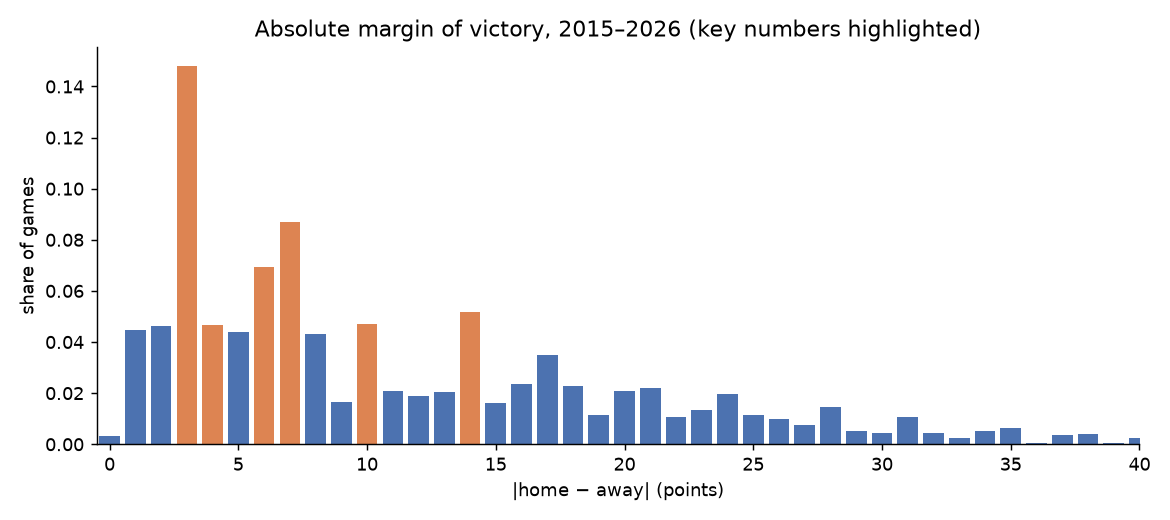
\includegraphics[width=0.95\textwidth]{nfl_abs_margin.png}
\caption{Absolute margin of victory, 2015--2026 (3,076 games); key numbers 3, 7, 6, 10 and 14 in orange.}
\label{fig:keynumbers}
\end{figure}

\begin{figure}[H]
\centering
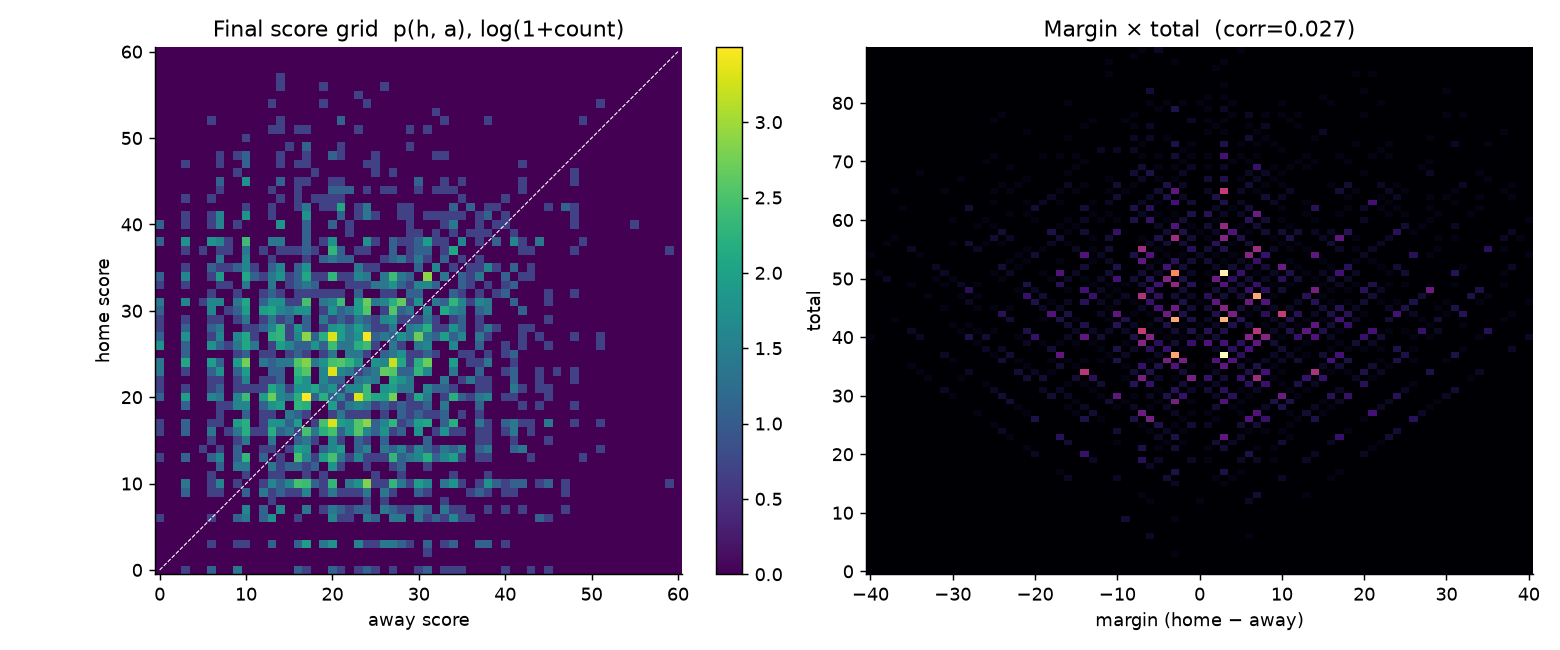
\includegraphics[width=0.95\textwidth]{nfl_score_grid.png}
\caption{Left: the empirical final-score grid $p(h,a)$ (log counts). Right: margin against total; the chequerboard is parity.}
\label{fig:scoregrid}
\end{figure}

\subsection{Positioning the empirical distribution for a game}

We want a distribution $p$ that (i) has the game's expected margin and total and (ii) is otherwise as close as possible to the historical prior $p_0$. Minimising the Kullback--Leibler divergence $\mathrm{KL}(p\,\|\,p_0)$ subject to the two moment constraints gives the exponential-family solution
\begin{equation}
p(h,a) \;\propto\; p_0(h,a)\,\exp\!\big(\lambda_1 (h-a) + \lambda_2 (h+a)\big),
\label{eq:tilt}
\end{equation}
with $(\lambda_1,\lambda_2)$ solved so that $\mathbb{E}[h-a]$ and $\mathbb{E}[h+a]$ match the targets, a two-equation root find. Because the tilt only reweights cells, it cannot create mass where the prior has none: a 3-point win stays 2.9 times as likely as a 4-point win. A Poisson or normal model would have to be taught key numbers, parity and cell clustering; the empirical grid already has them.

\paragraph{Worked example.} Pittsburgh at Cleveland, 1 October 2026, with the live Kalshi order book captured the day before (46 contracts). The sportsbook line was Cleveland $-2.5$ and total 38.5. Tilting the 3,076-game prior to those two numbers gives $\lambda_1=-0.0222$, $\lambda_2=-0.0399$ (Figures~\ref{fig:toy_dist} and~\ref{fig:toy_grid}). Table~\ref{tab:toy} compares model prices with the Kalshi mid for every contract.

\begin{figure}[H]
\centering
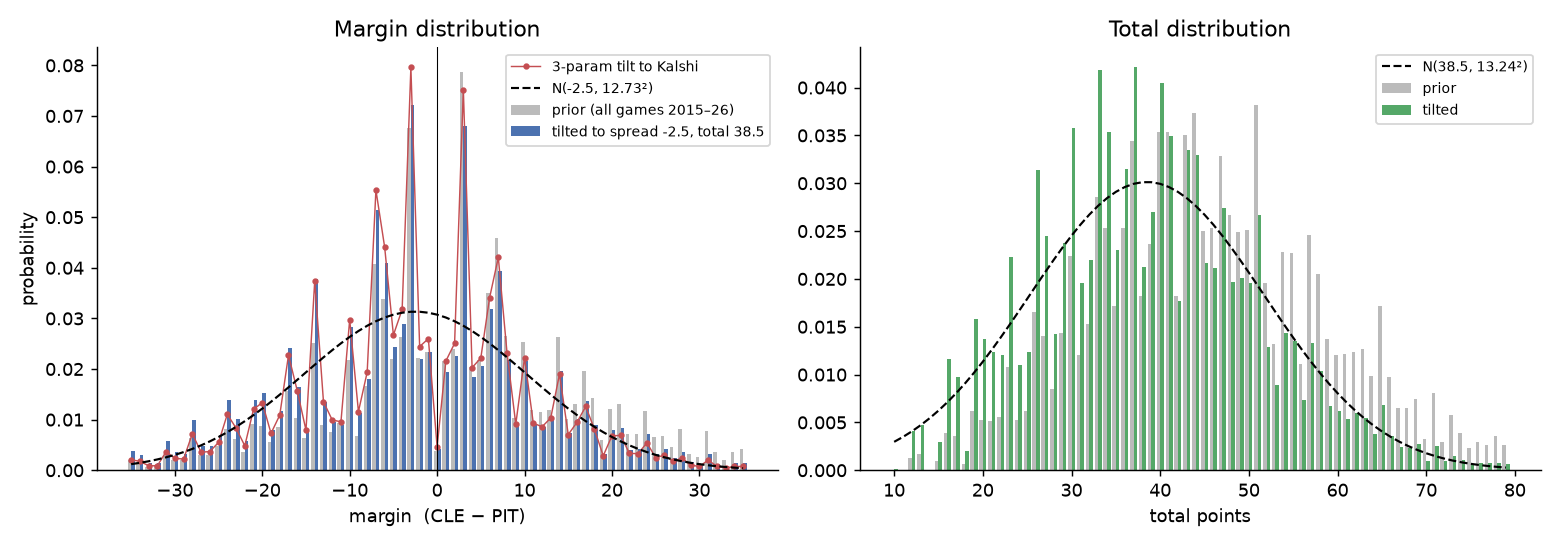
\includegraphics[width=0.98\textwidth]{toy_margin_total.png}
\caption{Margin (left) and total (right) distributions: grey the prior, blue the prior tilted to the book line, red a three-parameter tilt calibrated to Kalshi, dashed the normal.}
\label{fig:toy_dist}
\end{figure}

\begin{figure}[H]
\centering
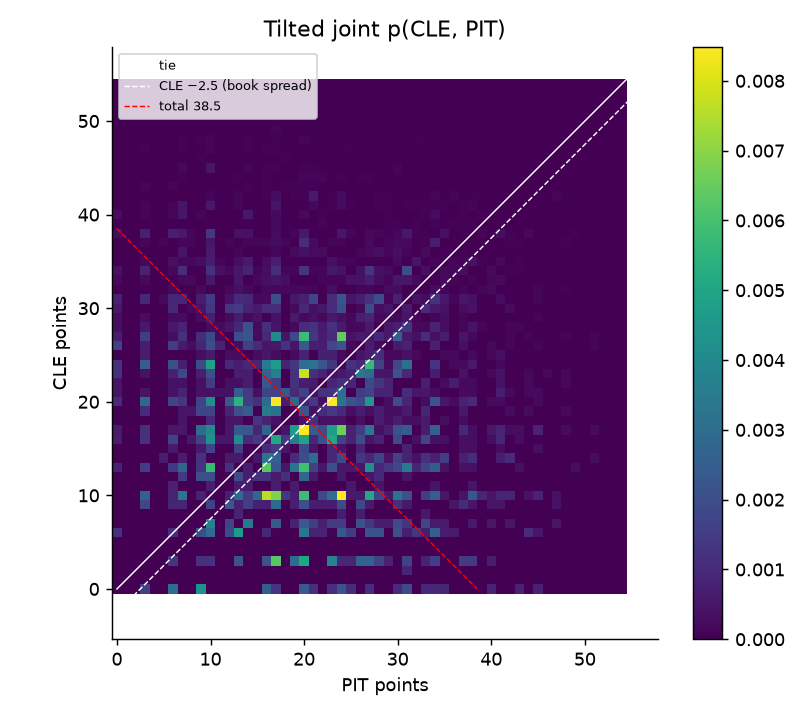
\includegraphics[width=0.6\textwidth]{toy_joint_grid.png}
\caption{The tilted joint table for Pittsburgh at Cleveland. The diagonal is a tie, the dashed line the book spread and the red line the total; each contract is a sum over one side of one of these lines.}
\label{fig:toy_grid}
\end{figure}

\begin{table}[H]
\centering
\small
\begin{tabular}{lcccc}
\toprule
\textbf{Model} & \textbf{All 46} & \textbf{Winner} & \textbf{Spread strikes} & \textbf{Total strikes} \\
\midrule
Untilted prior & 11.2 & 12.5 & 8.7 & 14.3 \\
Normal around the line & 1.89 & 0.28 & 2.32 & 1.48 \\
Tilt to the book line (no Kalshi data) & 1.52 & 0.08 & 1.98 & 1.06 \\
Two-parameter tilt fitted to Kalshi mids & 1.49 & 0.76 & 2.00 & 0.88 \\
Three-parameter tilt (adds margin$^2$) fitted to Kalshi & 0.76 & 0.24 & 0.64 & 0.99 \\
\bottomrule
\end{tabular}
\caption{Mean absolute error in cents of model price against the Kalshi mid, Pittsburgh at Cleveland. Quoted bid--ask spreads were 1--2 cents.}
\label{tab:toy}
\end{table}

\begin{figure}[H]
\centering
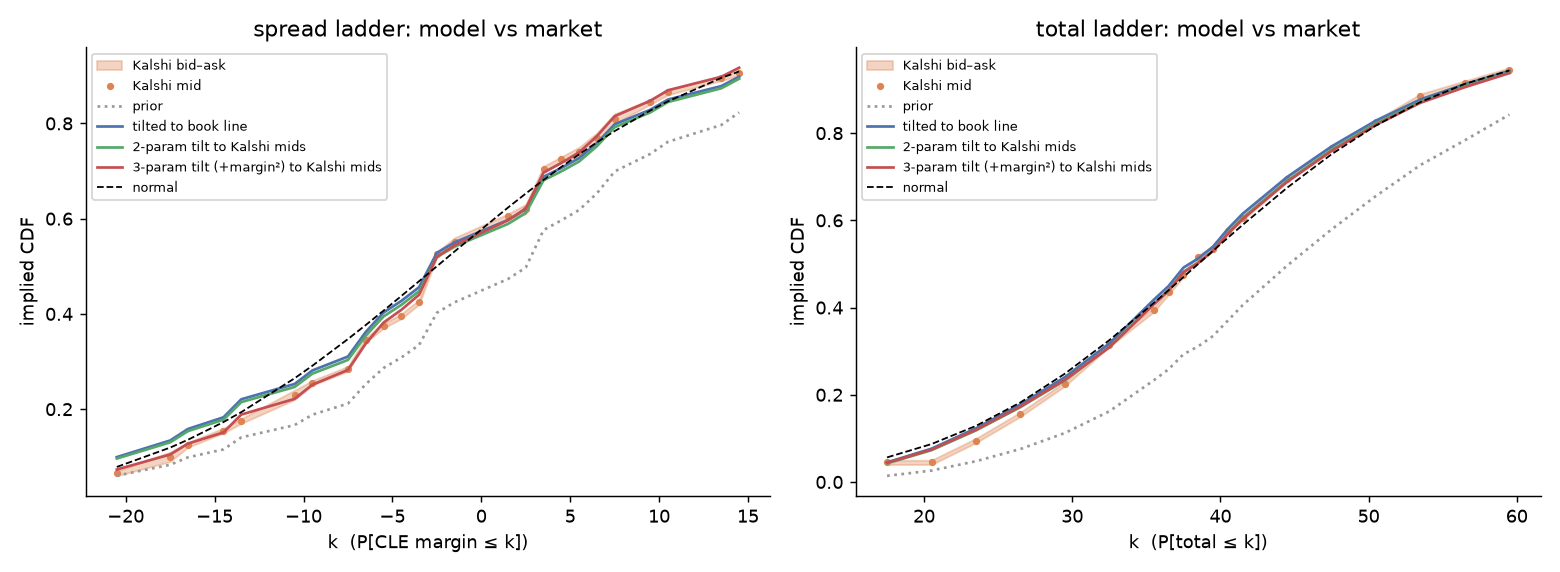
\includegraphics[width=0.98\textwidth]{toy_ladders.png}
\caption{Market-implied cumulative distributions from the spread (left) and total (right) ladders against the model variants. The shaded band is the Kalshi bid--ask.}
\label{fig:toy_ladders}
\end{figure}

Three lessons follow. Locating the distribution with the book line removes 87\% of the pricing error and prices the winner contract to 0.1 cents. Discreteness matters on the ladder: the normal is off by up to 6 cents on a single strike. And two moments do not control the tails: the book-tilted grid overprices Pittsburgh blowouts by 2--4.5 cents because the prior's margin has standard deviation 14.2 while the market prices this low-scoring game nearer 12.3. A third parameter on $(h-a)^2$ lets the market set the dispersion and the tail error disappears. This is the strongest argument for a model that predicts dispersion as well as location, and it motivates the score model of Section~\ref{sec:scoremodel}.

\subsection{What moves a game's expected score}

Before building features we listed the factors practitioners weigh when setting a line (Table~\ref{tab:factors}); the feature table of Section~\ref{sec:data} covers all but travel distance.

\begin{table}[H]
\centering
\small
\begin{tabular}{p{3cm}p{2.4cm}p{8.4cm}}
\toprule
\textbf{Factor} & \textbf{Typical effect} & \textbf{Notes} \\
\midrule
Starting quarterback & $\pm$3 to 10 pts & The largest single factor; elite starter versus backup is worth 7--10 points or 20--25 percentage points of win probability. Status should be modelled as a probability when questionable. \\
Team strength & baseline & Elo or power ratings, or EPA per play and success rate on offence and defence; adjust for opponent and regress toward the mean early in the season. \\
Home field & 1.5 to 2 pts & Has shrunk over the past decade; varies by venue and travel. \\
Other key injuries & 0.5 to 2 pts each & Costliest at offensive tackle, edge rusher, top cornerback and top receiver; multiple injuries on one unit compound. \\
Rest and schedule & 0.5 to 1.5 pts & Bye week helps; short week and long road trips hurt; time-zone changes matter for early-kickoff West Coast teams. \\
Weather and venue & totals & Wind above 15 mph and heavy precipitation suppress scoring; lowers the total and compresses variance. Domes remove it. \\
Coaching & 0.5 to 1 pt & Fourth-down aggressiveness, clock management, in-game adjustments. \\
Motivation and context & small, noisy & Playoff seeding, eliminated teams and week-18 rest can matter in specific spots. \\
Turnover luck & shrinkage & Fumble recoveries and close-game records are largely noise; use them to shrink apparent strength. \\
\bottomrule
\end{tabular}
\caption{Factors in a game's expected score, with typical magnitudes as cited by practitioners.}
\label{tab:factors}
\end{table}
